\chapter{Introducción}

El objetivo de este proyecto es evitar que un sistema \textit{blockchain} sea vulnerable a futuros ataques cuánticos. Para ello se ha implementado un algoritmo criptográfico resistente a ordenadores cuánticos, denominado UOV, para la firma de documentos, y posteriormente integrarlo en la \textit{blockchain} ARK.

\section{Motivación y contexto del proyecto}
\label{sec:intro:motivacion} %Esto se pone si queremos hacer referencia a esta sección

%En esta parte es importante clarificar las siguientes preguntas: 
%\begin{enumerate}
%\item ¿Cuál es el problema que pretendemos resolver con este proyecto? Debemos introducir un poco el contexto en el que aparece y describir bien en qué consiste dicho problema. 
%\item ¿Por qué es importante dicho problema? Hay que tratar de aportar datos y argumentos para indicar que el problema descrito es relevante en el contexto actual. 
%\end{enumerate}

La tecnología ha transformado nuestra sociedad en una sociedad digitalizada, donde actualmente, los dispositivos digitales comportan la mayor parte de nuestras actividades diarias en distintos ámbitos, como pueden ser actividades económicas, organizativas o sociales. En el proceso de digitalización de la sociedad podemos distinguir las siguientes cinco fases \cite{fases-digitalizacion}.\\

La primera fase o era del Internet, corresponde a mediados de los 90. En esta fase se comenzaron a crear páginas web para que los medios de comunicación y las empresas puedieran publicar y compartir información.

La segunda fase o era de las redes sociales, tuvo mayor auge a partir de 2005. Plataformas de bajo o ningún coste, se utilizaban en las empresas para poder llegar mejor a los clientes.

La tercera fase o era de la economía colaborativa, nació con la crisis de  2008 cuando las empresas tenían pocos recursos. Surgieron plataformas para conectar a las personas, y poder obtener lo que necesitasen unas de otras. Por ejemplo pagos online, ver recomendaciones y reseñas de un alojamiento o pedir un taxi. Además se da un gran paso ya que estas aplicaciones pasan de estar  alojadas en ordenadores a teléfonos inteligentes.

La cuarta fase o era del mundo autónomo, se ha desarrollado durante décadas. Se desarrollan tecnología con inteligencia artificial, es decir, que simulan la inteligencia de los humanos para poder resolver problemas más complejos.

Quinta fase o era del bienestar moderno, comienza con las pulseras inteligentes como \textit{Fitbit} o \textit{Fuelband} de Nike. Estas pulseras son el impulso de la tecnología para facilitar la vida de los clientes y poder integrar la tecnología en la vida de los mismos.\\

La digitalización debe de venir acompañada de mecanismos que aporten seguridad a los datos. Los pilares de la seguridad de la información son los conocidos como la tríada CIA (confidencialidad, integridad y  disponibilidad)\cite{servicios-seguridad}.\\

La \textbf{confidencialidad} es la propiedad que impide que la información pueda ser accesible por entidades no autorizadas. Un sistema garantiza la confidencialidad cuando un tercero entra en posesión de la información intercambiada entre el remitente y el destinatario, no es capaz de extraer ningún contenido legible. Para asegurar la confidencialidad se utilizan mecanismos de cifrado y ocultación de la comunicación.

La \textbf{integridad} busca mantener la exactitud de los datos, es decir, que no hayan sido modificados durante su envío. La integridad se obtiene adjuntando al mensaje otro conjunto de datos de comprobación de la integridad, un ejemplo es la firma digital.

La \textbf{disponibilidad} es la cualidad de la información de encontrarse a disposición de quienes deben acceder a ella, ya sean personas, procesos o aplicaciones, en el momentos que así lo quieran. Los mecanismos para asegurar la disponibilidad se implementan con la infraestructura tecnológica.\\

Además de estos tres pilares hay otro principio, la \textbf{autentificación}, que es la propiedad que permite identificar al generador de la información. Trata de comprobar si un mensaje enviado por un usuario, ha sido verdaderamente firmado por él mismo. Esto se consigue con el uso de cuentas de usuario y contraseñas de acceso.\\

Para garantizar estos servicios de seguridad se hace uso de protocolos de seguridad de la información entre los que se encuentra la criptografía, la lógica y la autenticación.\\

La criptografía se ocupa de cifrar ciertos mensaje con el fin de hacerlos ilegibles a receptores no autorizados, una vez que llega a su destino y sea descifrado, el receptor obtendrá el mensaje original \cite{criptografia}. Además dota de seguridad a las comunicaciones, a la información y a las entidades que se comunican.

Podemos diferenciar dos tipos de criptografía, la criptografía simétrica y la asimétrica. La criptografía simétrica utiliza la misma clave para cifrar y descrifrar un mensaje, esta clave la ha de conocer tanto el emisor como el receptor. La criptografía asimétrica utiliza dos claves la pública y la privada.

En la criptografía asimétrica podemos diferenciar dos ramas \cite{criptografia-asimetrica}. Por un lado, el cifrado de clave pública, donde el emisor cifra el mensaje con la clave pública del destinatario y el receptor lo descifra con su propia clave privada. Y por otro lado, las firmas digitales, donde el emisor firma el mensaje con su clave privada y el receptor puede verificar el mensaje con su propia clave pública, además cualquier manipulación del mensaje se refleja en su resumen o \textit{hash}.\\

Este tipo de criptografía basa su seguridad en la hipótesis de que no se pueden encontrar las claves por fuerza bruta con la tecnología existente en la actualidad. Los ataque de fuerza bruta tratan de recuperar las claves probando todas las posibles combinaciones hasta encontrar la que permite el acceso, a partir del algoritmo de cifrado y del texto cifrado con su original \cite{fuerza-bruta}. Para que la búsqueda tenga éxito se deberán de realizar $10^n-1$ operaciones donde $n$ es la logitud de la clave. 

Otro factor importante es si en la clave aparencen números, caractéres o la combinación de ambos, aumentando así el coste de encontrar las clavess, llegando a alcanzar tiempos de cálculo logarítmicos, es decir, que podrían tardar siglos en encontrar una contraseña compleja pero también depende de la capacidad de operación del ordenador.\\

En este contexto, la aparición de la futura computación cuántica permitirá el cálculo de operaciones a una velocidad mucho mayor. En la gráfica \ref{fig:comp-clasica-cuantica} podemos observar la capacidad de cómputo del peor ordenador cuántico, con la línea continua, que sigue la gráfica de una función exponencial, frente a la capacidad del mejor ordenador clásico, la línea discontinua, que sigue una función lineal.

\begin{figure}[h]
	\centering
	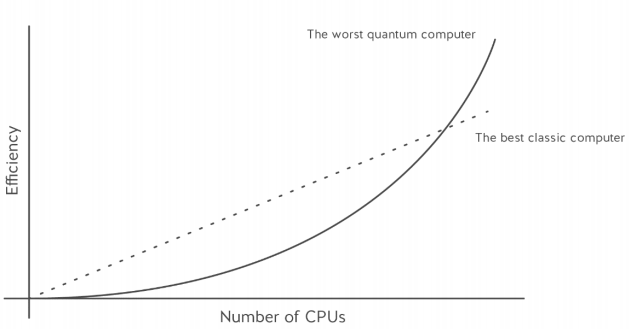
\includegraphics[width=0.8\textwidth]{figuras/comp_clasica_cuantica.png}
	\caption{Comparativa de la capacidad de cómputo de un ordenador clásico con un ordenador cuántico\cite{clasica-vs-cuantica}}
	\label{fig:comp-clasica-cuantica}
\end{figure}

La comparativa también nos muestra que para operaciones pequeñas como, por ejemplo, editar un documento de texto un ordenador cuántico sería probablemente ineficienciente. Por tanto lo mejor sería un ordenador híbrido, que mezclase computación clásica, para cálculos pequeños, y computación cuántica, para operaciones de mayor tamaño.\\

Cuando esté desarrollado el ordenador cuántico no serán válidos los actuales algoritmos criptográficos de clave pública, como RSA, Diffie-Hellman y ECDSA, ya que se basan en los problemas del logaritmo discreto y factorización de enteros, resolubles fácilmente por un ordenador cuántico. Veámos una tabla comparativa\ref{table:security-level}, nos indice \\

\begin{table}[h]
	
	\label{table:security-level}
	\centering
	\resizebox{\linewidth}{!}{
	\begin{tabular}{c c c c c }
		\hline \\[-1.5ex]
		\thead{Tipo} & \thead{Algoritmo-Longitud clave} & \thead{Nivel seguridad\\ (ordenador clásico)} & \thead{Nivel seguridad\\ (ordenador cuántico)} & \thead{Ataque cuántico}\\ [1ex] 
		\hline\hline \\[-1.5ex]
		\multirow{4}{5em}{Asimétrico} & RSA-2048 & 112 & 0 & Algoritmo de Shor \\ [0.5ex]
		& RSA-3072 & 128 & 0 & Algoritmo de Shor \\ [0.5ex]
		& ECC-521 & 128 & 0 & Algoritmo de Shor \\ [0.5ex]
		& ECC-521 & 256 & 0 & Algoritmo de Shor \\ [0.5ex]
		\hline
		\multirow{2}{5em}{Simétrico} & AES-128 & 128 & 64 & Algoritmo de Grover \\ [0.5ex]
		& AES-256 & 256 & 128 & Algoritmo de Grover \\ [1ex]
		\hline
	\end{tabular}}
	\caption{Niveles de seguridad de ordenadores clásicos y cuánticos \cite{security-bit}}
\end{table}


En la actualidad, se están desarrollando muchos algoritmos para que sean resistentes a ataque de tipo cuántico.\\

Por otro lado, también en la actualidad está siendo muy relevante la adopción de las blockchain como tecnología para ofrecer diversos servicios.\\

En este proyecto, hemos implementado un algoritmo resistente a ataques cuánticos, UOV \cite{algoritmo-UOV} y se ha adaptado a la \textit{blockchain} ARK para que se utilice dicho algoritmo de firma.\\

El agoritmo de firma implementado en la \textit{blockchain} es Schnorr basado en el problema del logaritmo discreto, por eso lo hemos modificado.

\section{Objetivos del proyecto y logros conseguidos}
\label{sec:intro:objetivos}
El objetivo de este proyecto es modificar el algoritmo de firma y verificación de las transacciones de la \textit{blockchain} ARK, para hacerla resistente a ataques cuánticos.

\begin{itemize}
	\item Implementación del algoritmo UOV: Se ha implementado las funciones de generación de claves tanto públicas como privadas, la función de firma a partir de la clave privada y la función de verificación de la misma con la clave pública. Además ha sido necesario implementar la aritmética de cuerpo finito de $2^7$ elementos.
	\item Integrar el algoritmo UOV en la \textit{blockchain} ARK para comprobar su funcionamiento: Se ha modificado el algoritmo de firma dado en la \textit{blockchain} por el algoritmo UOV para aumentar la seguridad.

\end{itemize}


\section{Estructura de la memoria}
%Se describirán los capítulos que tiene la memoria, indicando qué contenidos habrá en cada uno de ellos, para permitir al lector situarse ante el documento. 

A continuación se muestran los capítulos que presenta la memoria junto con una breve descripción de lo que contiene cada uno.

\begin{enumerate}
	\item Introducción: Presenta la motivación del proyecto, con una introducción a la computación cuántica y la \textit{blockchain}. También encontramos los objetivos que se persiguen con este trabajos.
	\item Planificación y costes: Definición de las entregas y seguimiento del proyecto. Además incluye el presupuesto del proyecto.
	\item Análisis del problema: Descripción de las funcionalidades y requisitos, y análisis de los objetivos que se muestran en la sección \ref{sec:intro:objetivos}.
	\item Diseño: En esta sección podemos encontrar el diseño de la implementación del algoritmo UOV y el diseño del ecosistema ARK, donde integraremos el algoritmo.
	\item Implementación: Se explicará el código de la implementación del algoritmo UOV y la aritemética implementada para el cuerpo finito de $2^7$ elementos.
	\item Evaluación y pruebas: Ejemplo de la firma de una transacción en el sistema ARK.
	\item Conclusiones
\end{enumerate}

\section{Contenidos teóricos para la comprensión del proyecto}

En los siguientes apartados se explica los contenidos claves de este proyecto.

\subsection{Computación cuántica}

\subsection{Algoritmo UOV}

\subsection{Blockchain}



\begin{itemize}
	\item Algoritmo cuántico: Son los algoritmos que pueden ser resueltos por un computador cuántico en tiempo polinómico.

	%\item Contratos inteligentes: Base de "propiedades inteligentes" que permiten definir mediante códigos de la Blockchain, la forma en la que los dispositivos reaccionan ante eventos que tienen lugar en su entorno. Llevan incorporada una máquina virtual que habilita la codificación y ejecución de programas software para determinar las condiciones sobre el intercambio de activos entre agentes.


 	\item Firma electrónica: Sirve para controlar la integridad de los datos y asegurar que la información procede de quien dice ser su remitente, garantiza que la información que se almacena o se envía no ha sido modificada. Controla la auditoría del documento \cite{firmaDigital}. 


	\item Criptosistemas asimétricos: Cada usuario posee una clave pública y otra privada. El usuario cifrará con la clave privada del usuario y descifrará con la clave pública del usuario que haya mandado el mensaje, que previamente se la habrá mandado a dicho usuario. En algunos criptosistemas se utilizan claves compartidas que se calculan a partir de la clave privada de un usuario A y la clave pública de un usuario B. El algoritmo UOV es de este tipo, es decir, que necesitaremos claves privadas y públicas para firmar y verificar las firmas.


	\item Resumen o \textit{Hash}: Es el resultado de aplicar una función que transforma un mensaje que longitud variable en uno de longitud fija, denominada función hash. Es el resultado de calcular el resto módulo n con n la longitud fija. Al aplicar la función hash a un fichero, si se modifica algún dato del mismo cambiará su hash y por tanto se sabrá si ha sido manipulado desde que se envió. Así podemos conseguir la integridad del mensaje


	\item \textit{Blockchain}: Sistemas de almacenamiento de información que se divide en bloque de datos enlazados mediante los hash. A cada bloque se le asocia un hash a partir del bloque anterior, creando una lista enlazada, la búsqueda de información no es muy óptima si hay un número elevado de bloques. %Para la búsqueda eficiente en \textit{blockchain} se usan los árboles merkle.
	
\textit{Blockchain} por si mismo no soluciona los problemas de los sistemas de la información y la comunicación, pero permiten impulsar modificaciones orientadas a crear soluciones más robustas, implicando conocer donde hay que usar las \textit{blockchain} y cual es la infraestructura \cite{blockchain}.


	%\item Árboles Merkle: Árboles binarios con funciones hash, cada nodo tiene con máximo dos hijos, no hay ciclos. El cálculo de los hash de los padres se hace combinando los hash de los hijos. La integridad se obtiene inclueyendo en los bloques el valor del nodo raíz en lugar de añadir el valor de todos los datos protegidos por los bloques, reducimos además la información de la cabecera.
	
	
	A lo largo del desarrollo de este trabajo tendremos presentes dos tecnologías, la computación cuántica y las cadenas de bloques. 

La computación cuántica constituye un nuevo paradigma de la informática basado en los principios de la teoría cuántica. La computación clásica funciona con bits cuyos valores pueden ser 0 o 1, mientras que la computación cuántica funciona con bit cuánticos o cúbits, donde son una combinación de 0 y 1, pudiendo tomar ambos valores a la vez, esto se denomina la superposición cuántica de los estados \cite{computacioncuantica-criptografia}.
La figura \ref{fig:bit-cubit} muestra

\begin{figure}[h]
	\centering
	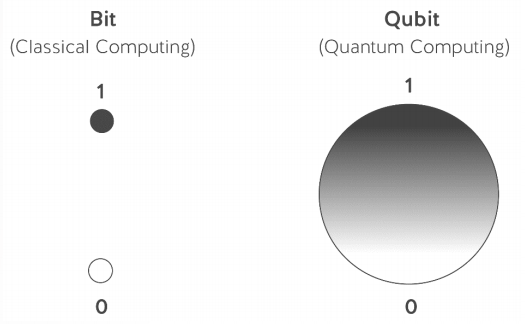
\includegraphics[width=0.8\textwidth]{figuras/bit_cubit.png}
	\caption{Comparativa de la capacidad de cómputo de un ordenador clásico con un ordenador cuántico\cite{clasica-vs-cuantica}}
	\label{fig:bit-cubit}
\end{figure}

La superposición cuántica aporta gran capacidad de procesamiento, lo que hace posible resolver de manera eficiente problemas de mayor complejidad como la factorización de enteros, el algoritmo discreto y la simulación cuántica, que a día de hoy con los ordenadores clásicos son difíciles de romper. 

Otro aspecto importante de la física cuántica relacionado con la superposición es el entrelazamiento de las partículas\cite{cumputacioncuanticaclasica}. Esto es, si dos partículas en algún instante han interactuado retienen un tipo de conexión y pueden entrelazarse formando pares. Esto permite que aunque los cúbits estén separados interactúen entre sí. Con estos dos aspectos la capacidad de procesamiento aumenta considerablemente, cuántos más cúbits la capacidad de procesamiento aumenta considerablemente.


La evolución de la tecnología se ha basado principalmente en la reducción de los transistores para aumentar la velocidad, llegando a escalas de tan solo algunas decenas de nanómetros. Esto tiene un límite y es la eficiencia, puesto que al seguir disminuyendo el tamaño podrían dejar de funcionar correctamente. De ahí surge la necesidad de descubrir nuevas tecnologías, la computación cuántica \cite{computacioncuanticawiki}.

El estudio de las tecnologías cuánticas se inició en 1980, donde surgieron teorías con la posibilidad de realizar cálculos cuánticos. En la década de los 90 se empezó a poner en práctica algunas teoría, apareciendo los primeros algoritmos cuánticos, primeras aplicaciones cuánticas y las primera máquinas diseñadas para realizar cálculos cuánticos.\\



Por otro lado tenemos las cadenas de bloques o \textit{blockchain}. Esta tecnología permite verificar, validar, rastrear todo tipo de información, ya sean contratos inteligentes, transacciones financieras, certificados digitales o firmas, que será el centro de este proyecto.

Los datos que almacenan cada bloque son transacciones válidas, información referente a ese bloque y la relación con el bloque anterior mediante el \textit{hash}, por tanto el bloque tiene un lugar específico dentro de la cadena. De esta forma si hay una alteración en un determinado bloque se verá reflejado en su \textit{hash} y en el de los bloques posteriores, haciendo que la cadena que la información de la cadena no se pueda perder, modificar o eliminar. 

Las aplicaciones de las cadenas de bloques son diversas entre ellas se encuentra la salud o la firma de documentos en las notarías. En el primer caso, cada centro  de salud podría tener el historial médico de cualquier paciente, de una forma segura y evitando falsificaciones, estos historiales se encontrarían en nodos distribuidos de forma descentralizada de forma que tuvieran un acceso rápido y seguro. En el segundo caso será en el que nos centraremos a lo largo de este proyecto. Hoy día la firma de documentos o transacciones por parte de un usuario es un problema puesto que se pueden copiar con facilidad, pero con \textit{blockchain} no podrían ser falsificadas debido a la propiedad de validación y rastreo de los datos.\\

Las \textit{blockchain} por si mismas serían vulnerables a ataques cuánticos, pues su única línea de defensa sería el algoritmo de firma de los bloques. Las cadenas de bloques actualmente son seguras, puesto que un ordenador clásico no tiene la capacidad de cómputo necesaria para descifrar cada bloque, obtener la información y volver a firmar todos los bloques sin dejar huella. Por eso para hacer una \textit{blockchain} resistente es necesario tener un criptosistema que no se pueda romper con computación cuántica, como por ejemplo el algoritmo UOV, ver sección \ref{sec:implementacion}. 

\end{itemize}


